% Functional Prediction
%
% A very simple overview of gene functional prediction

  \section{Functional Prediction}
    \begin{frame}
      \frametitle{Methods}   
      Most involve annotation transfer by sequence homology. \\
      Much is dependent on the quality of the alignment, and training set annotation.
      \begin{itemize}
        \item (Blast2GO \url{http://www.blast2go.com/b2ghome})
        \item (KEGG Automatic Annotation Server \url{http://www.genome.jp/kegg/kaas/})
        \item PFam \url{http://www.sanger.ac.uk/resources/databases/pfam.html}
        \item InterProScan \url{http://www.ebi.ac.uk/interpro/interproscan.html}
        \item RAST \url{http://rast.nmpdr.org/}
      \end{itemize}
    \end{frame}

    % PFam
    \subsection{PFam}
    \begin{frame}
      \frametitle{How PFam Works}   
      \begin{itemize}
        \item [PFam-A] Curators identify domains of interest (may or may not have known function)
        \item [PFam-B] Sequence segments (from the ADDA domain sequence database) that don't match PFam-A are automatically grouped into families
        \item A seed alignment is constructed from representative sequences
      \end{itemize}
      \begin{center}
        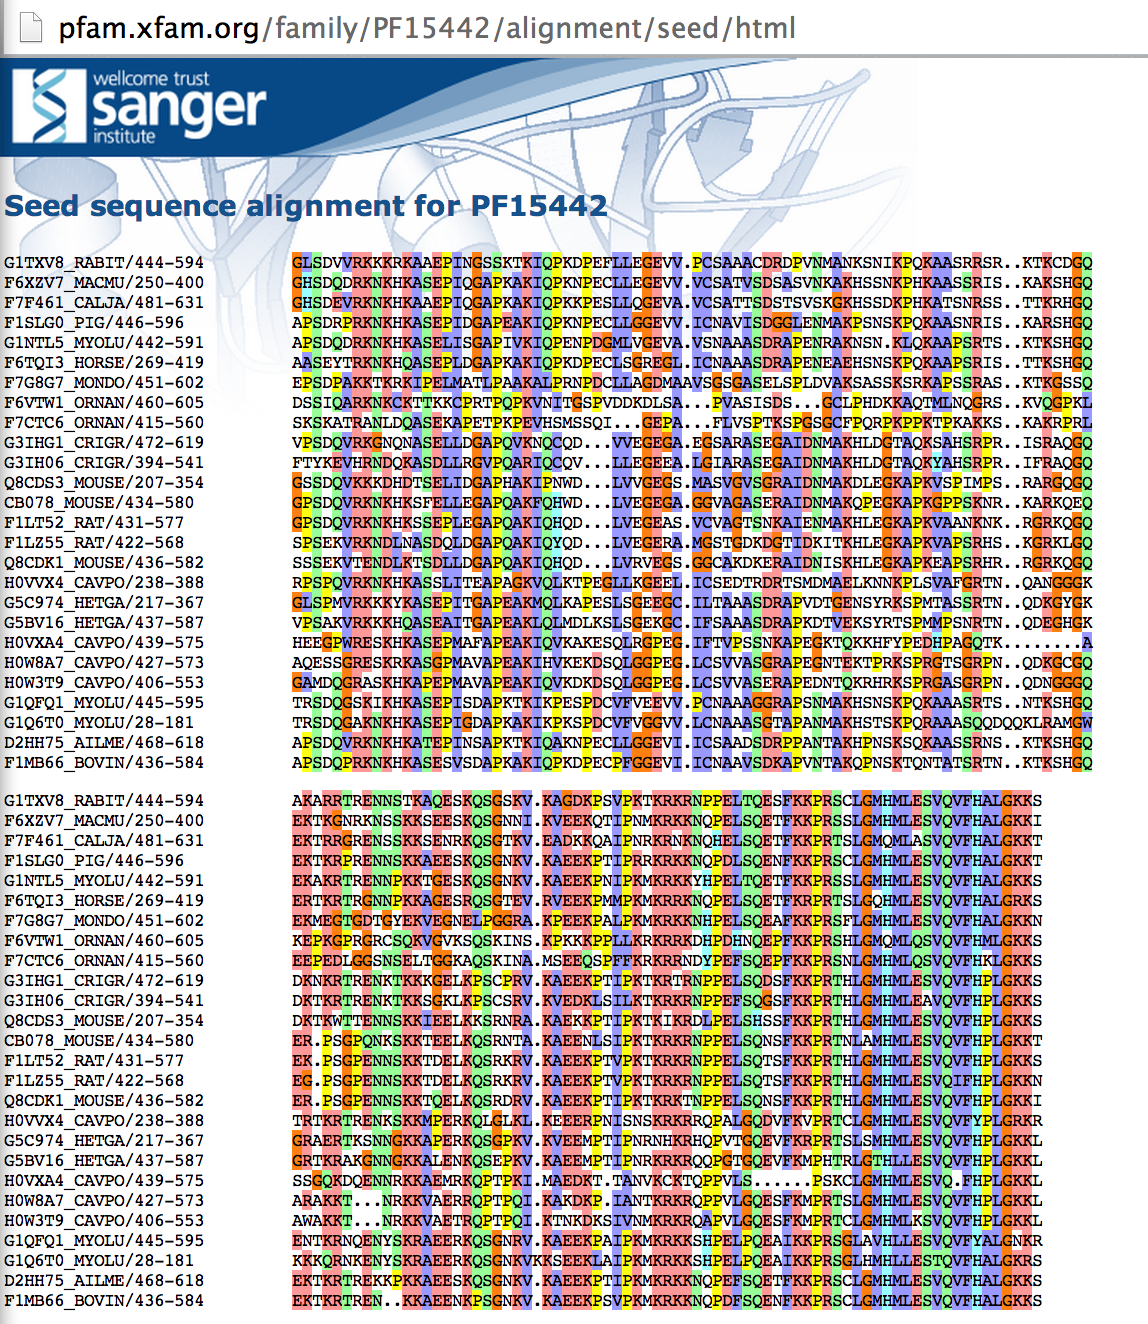
\includegraphics[width=0.3\textwidth]{images/pfam1}     
      \end{center}      
    \end{frame}

    \begin{frame}
      \frametitle{How PFam Works}   
      \begin{itemize}
        \item A profile HMM is built from the seed alignment, using HMMer
        \item Profile HMMs can be represented as sequence logos
      \end{itemize}
      \begin{center}
        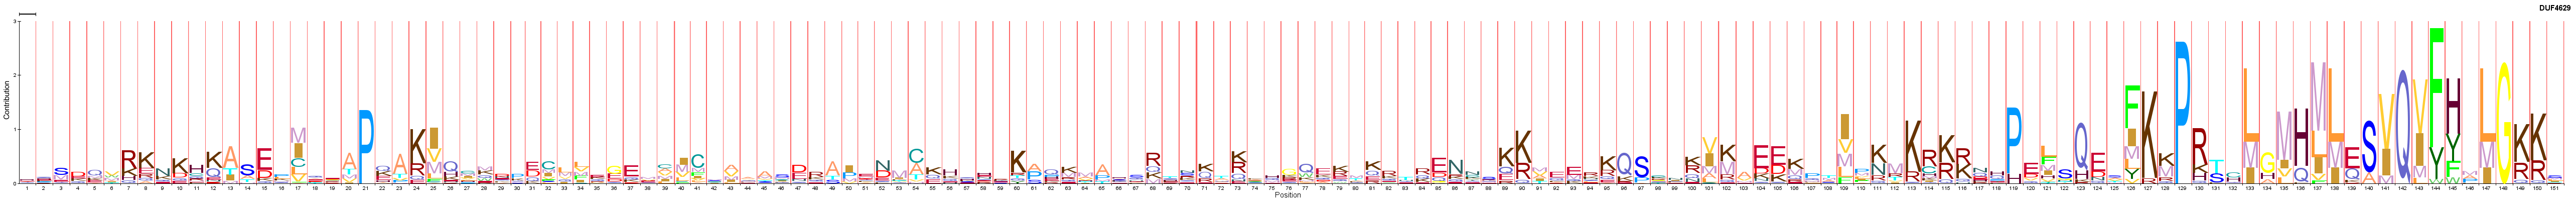
\includegraphics[width=0.9\textwidth]{images/pfam2} 
      \end{center}      
    \end{frame}

    \begin{frame}
      \frametitle{How PFam Works}   
      \begin{itemize}
        \item Profile HMM used to query several sequence databases, to generate full alignment
        \item Curated thresholds are used to determine family membership
      \end{itemize}
      \begin{center}
        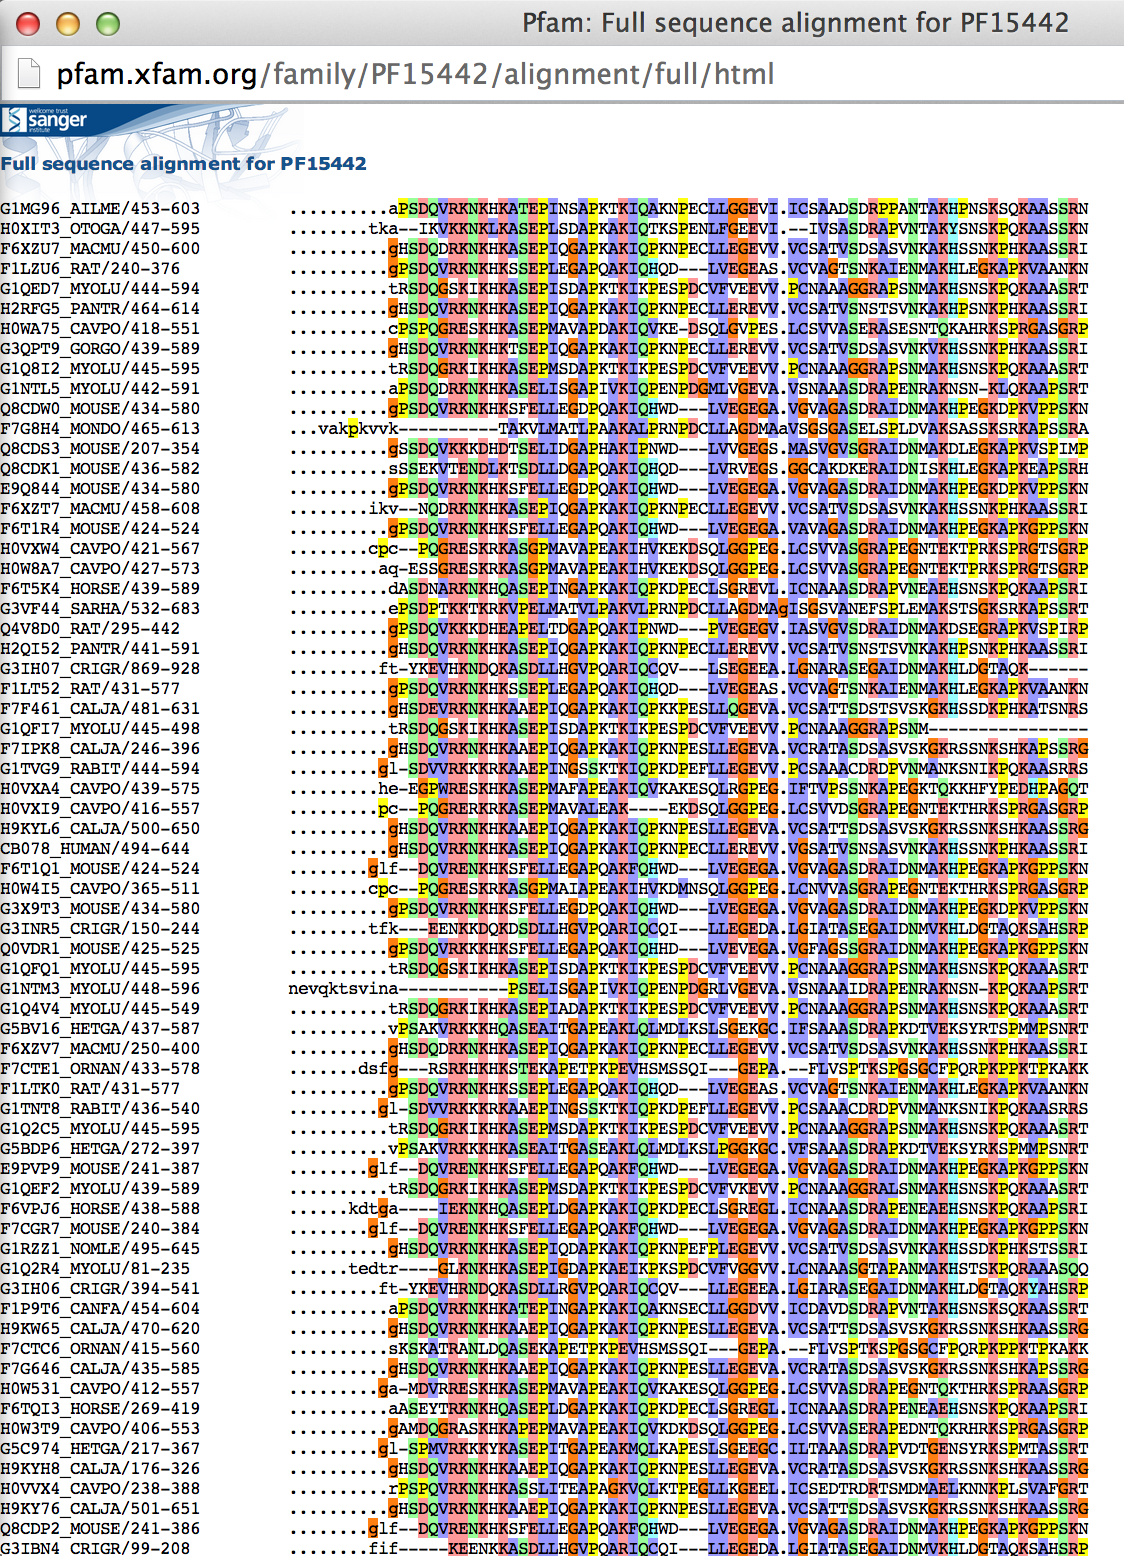
\includegraphics[width=0.3\textwidth]{images/pfam3} 
      \end{center}      
    \end{frame}

    \begin{frame}
      \frametitle{How PFam Works}  
      Bit score is used, not E-value
      \begin{itemize}
        \item [GA] Gathering threshold: Manually-determined for each family, used to build full alignment. Set to exclude false positives 
        \item [TC] Trusted cutoff: Lowest sequence score and domain score of match in the full alignment
        \item [NC] Noise cutoff: Highest sequence score and domain score of match not in full alignment
      \end{itemize}
      \begin{center}
        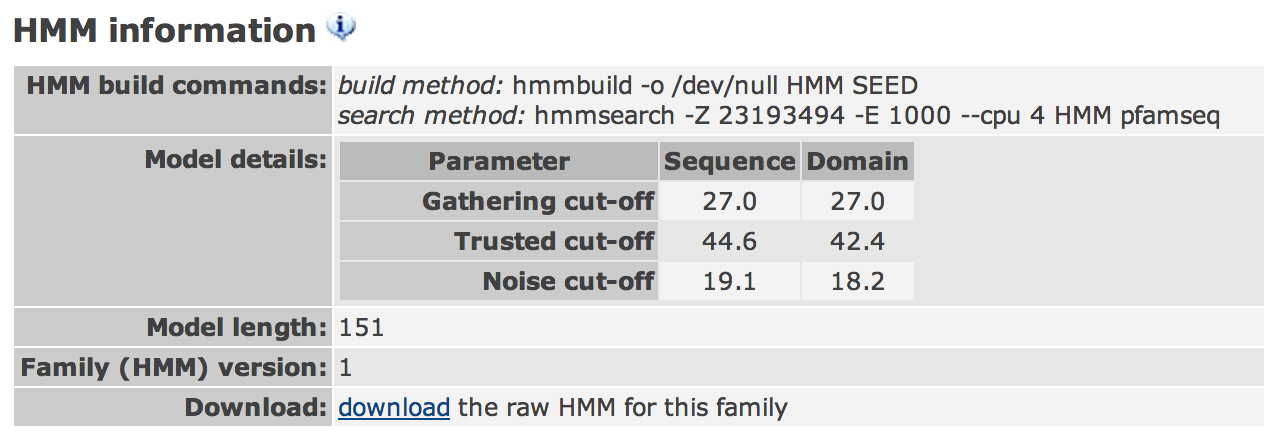
\includegraphics[width=0.5\textwidth]{images/pfam4} 
      \end{center}      
    \end{frame}

    \begin{frame}
      \frametitle{PFam example}  
      Choose a sequence from your annotated draft genome, in Artemis \\
      \begin{center}
        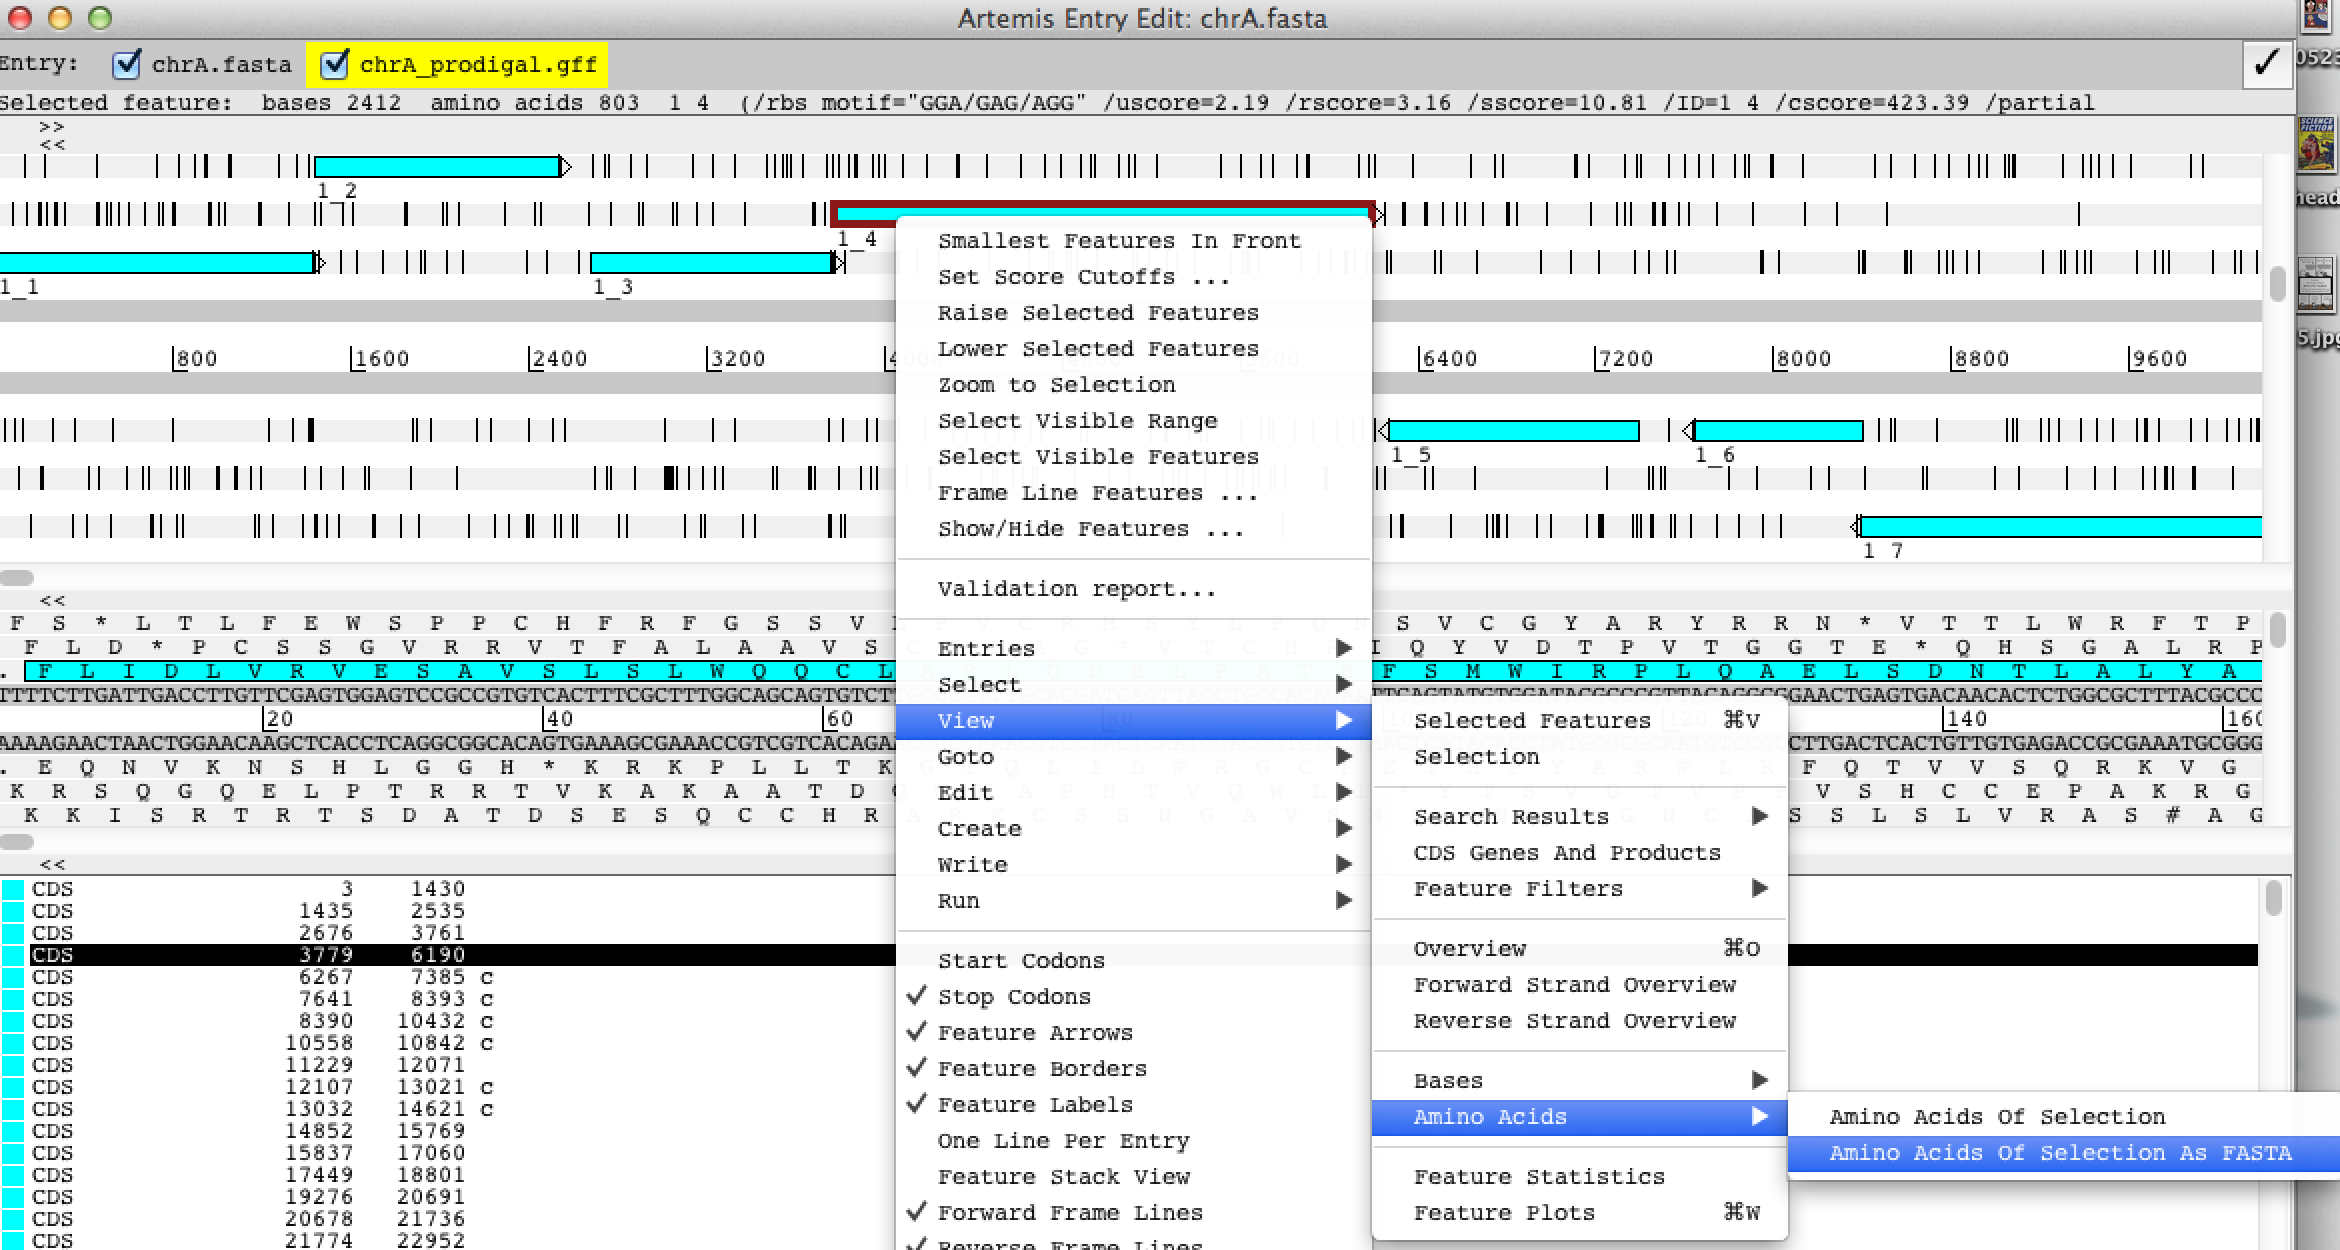
\includegraphics[width=0.9\textwidth]{images/pfam5} 
      \end{center}      
    \end{frame}

    \begin{frame}
      \frametitle{PFam example}  
      Copy the sequence to clipboard
      \begin{center}
        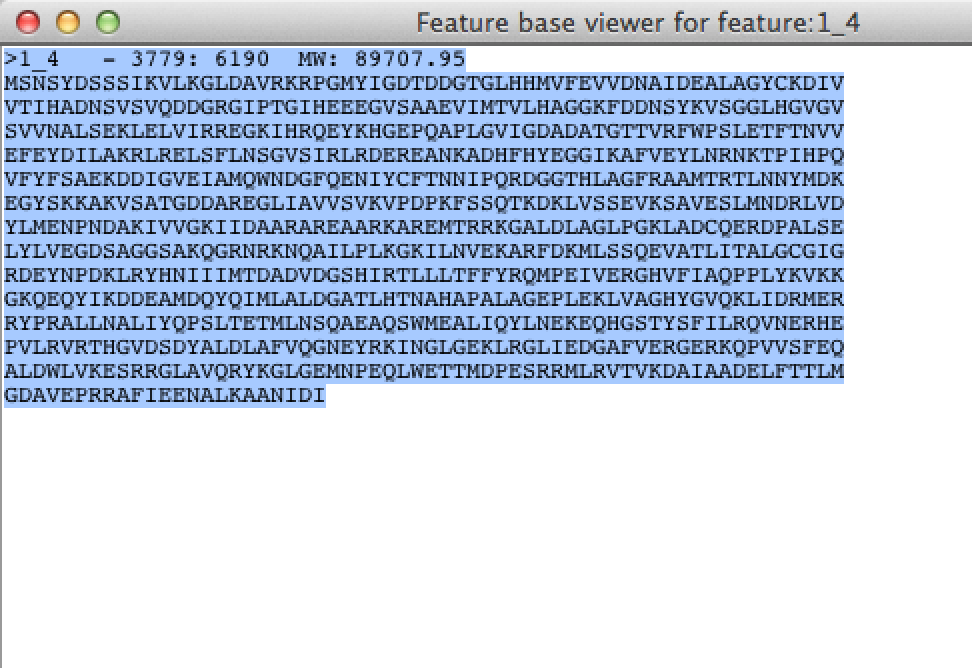
\includegraphics[width=0.5\textwidth]{images/pfam6} 
      \end{center}      
    \end{frame}

    \begin{frame}
      \frametitle{PFam example}  
      Open \url{http://pfam.xfam.org/} in your browser \\
      Click on "SEQUENCE SEARCH"
      \begin{center}
        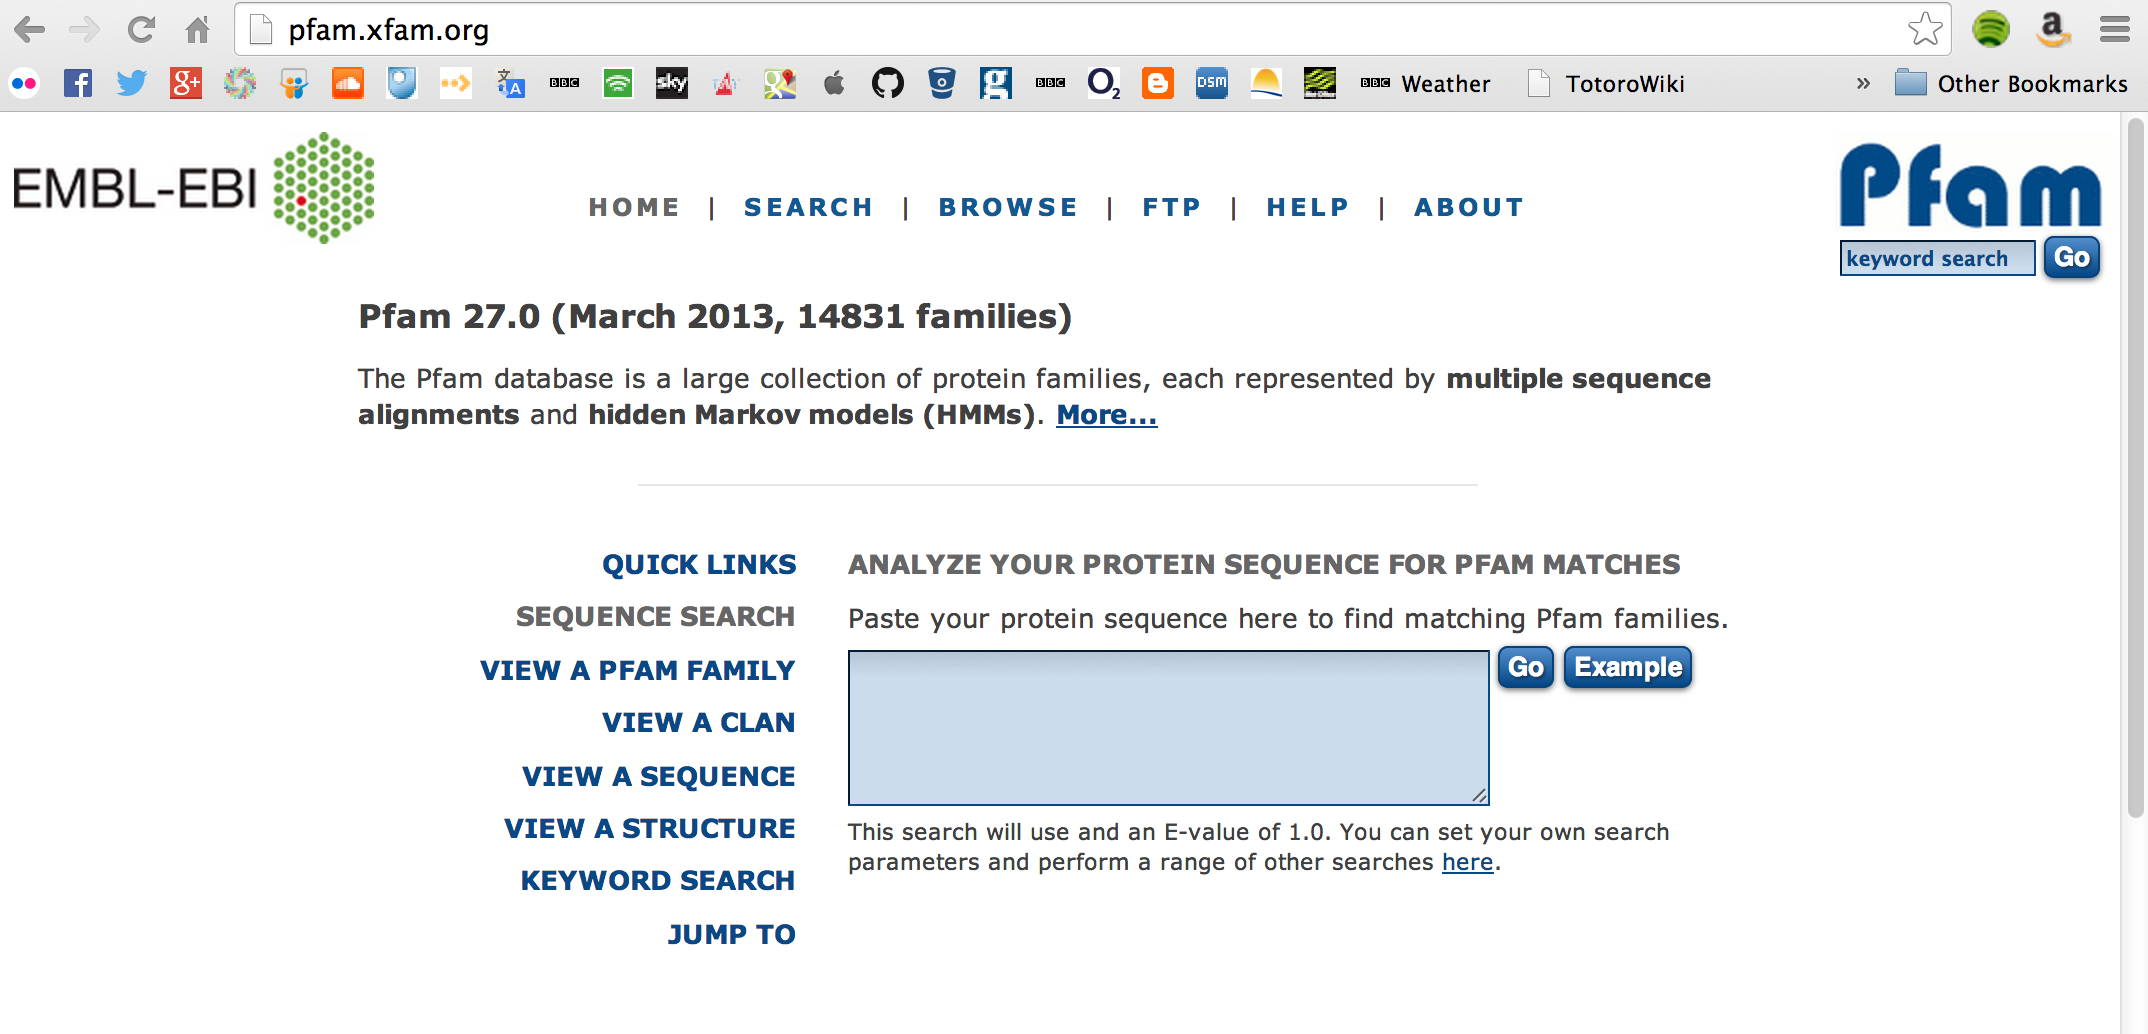
\includegraphics[width=0.9\textwidth]{images/pfam7} 
      \end{center}      
    \end{frame}

    \begin{frame}
      \frametitle{PFam example}  
      Paste your sequence and click "Go"
      \begin{center}
        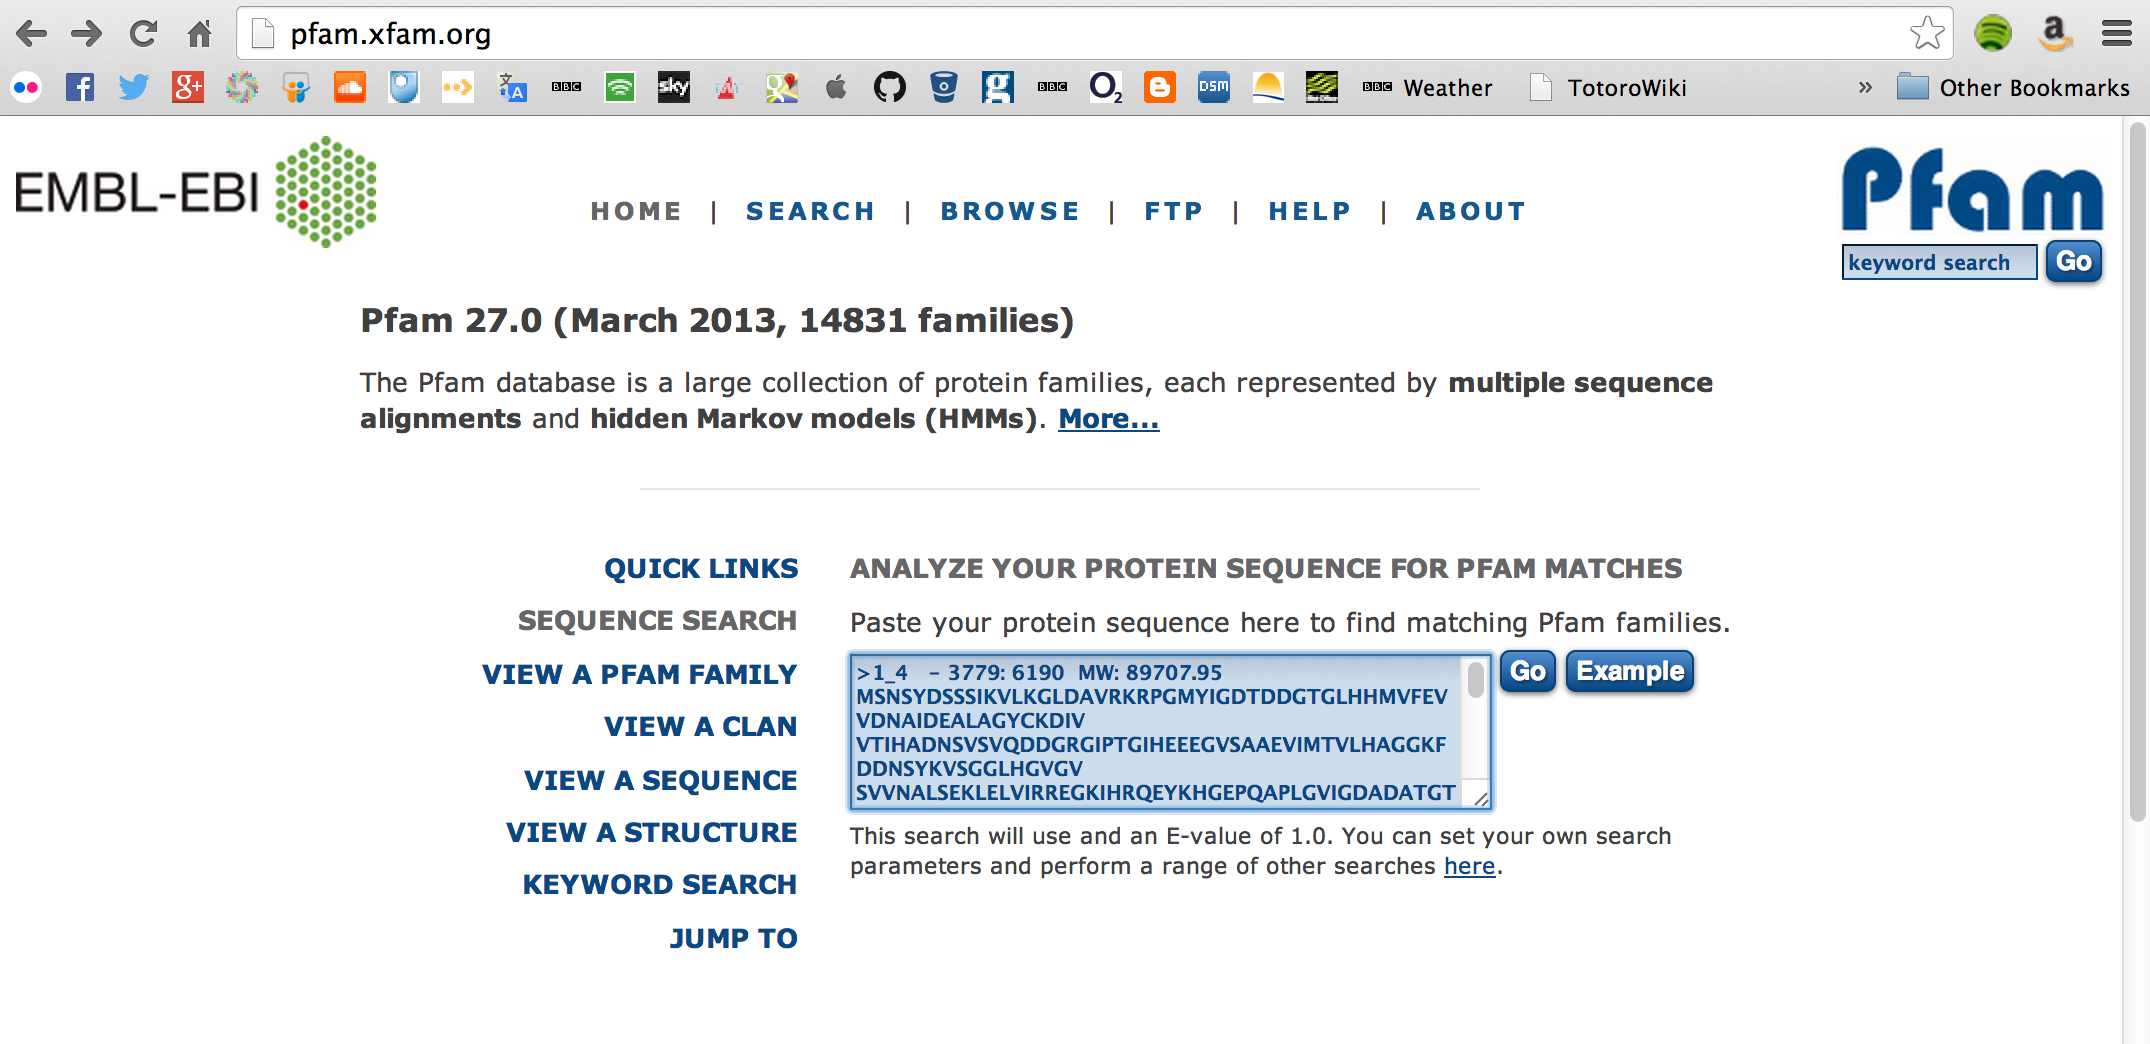
\includegraphics[width=0.9\textwidth]{images/pfam8} 
      \end{center}      
    \end{frame}

    \begin{frame}
      \frametitle{PFam example}  
      Domain matches are returned \\
      (but maybe not for your choice of CDS$\ldots$)
      \begin{center}
        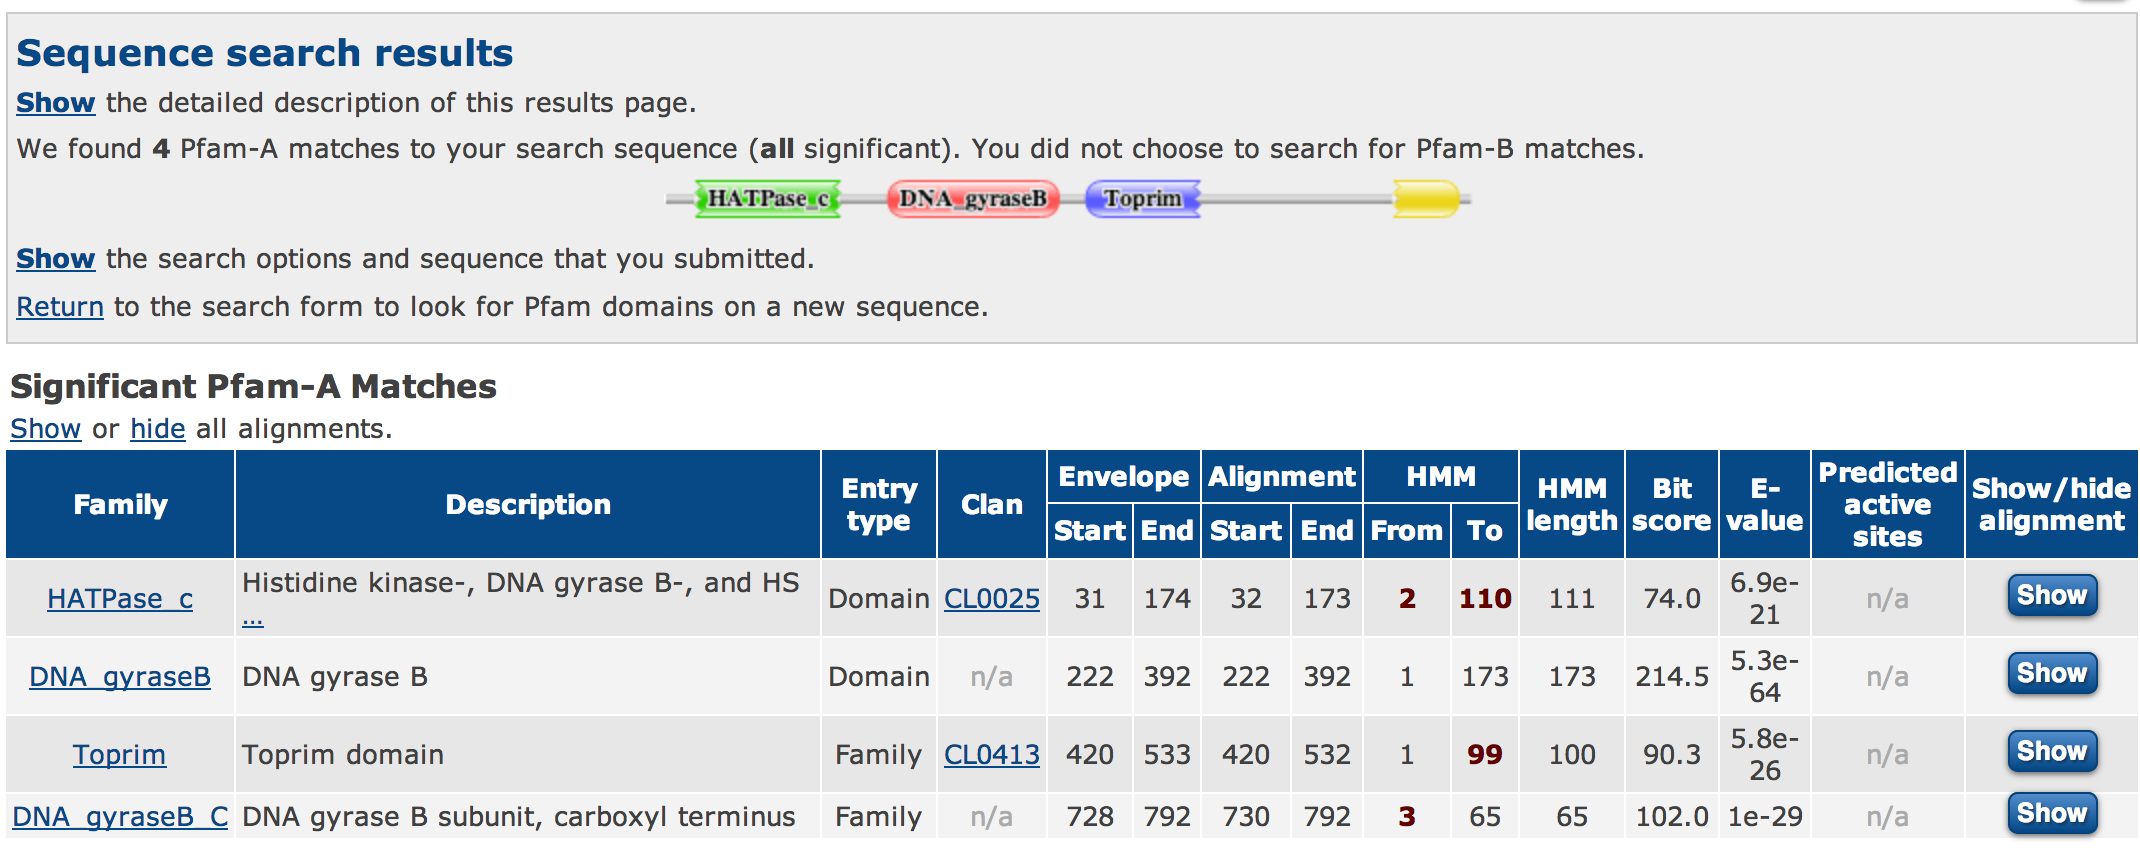
\includegraphics[width=0.9\textwidth]{images/pfam9} 
      \end{center}      
    \end{frame}

    \begin{frame}
      \frametitle{PFam example}  
      Compare match bit scores to GA, TC, NC thresholds for each domain
      \begin{center}
        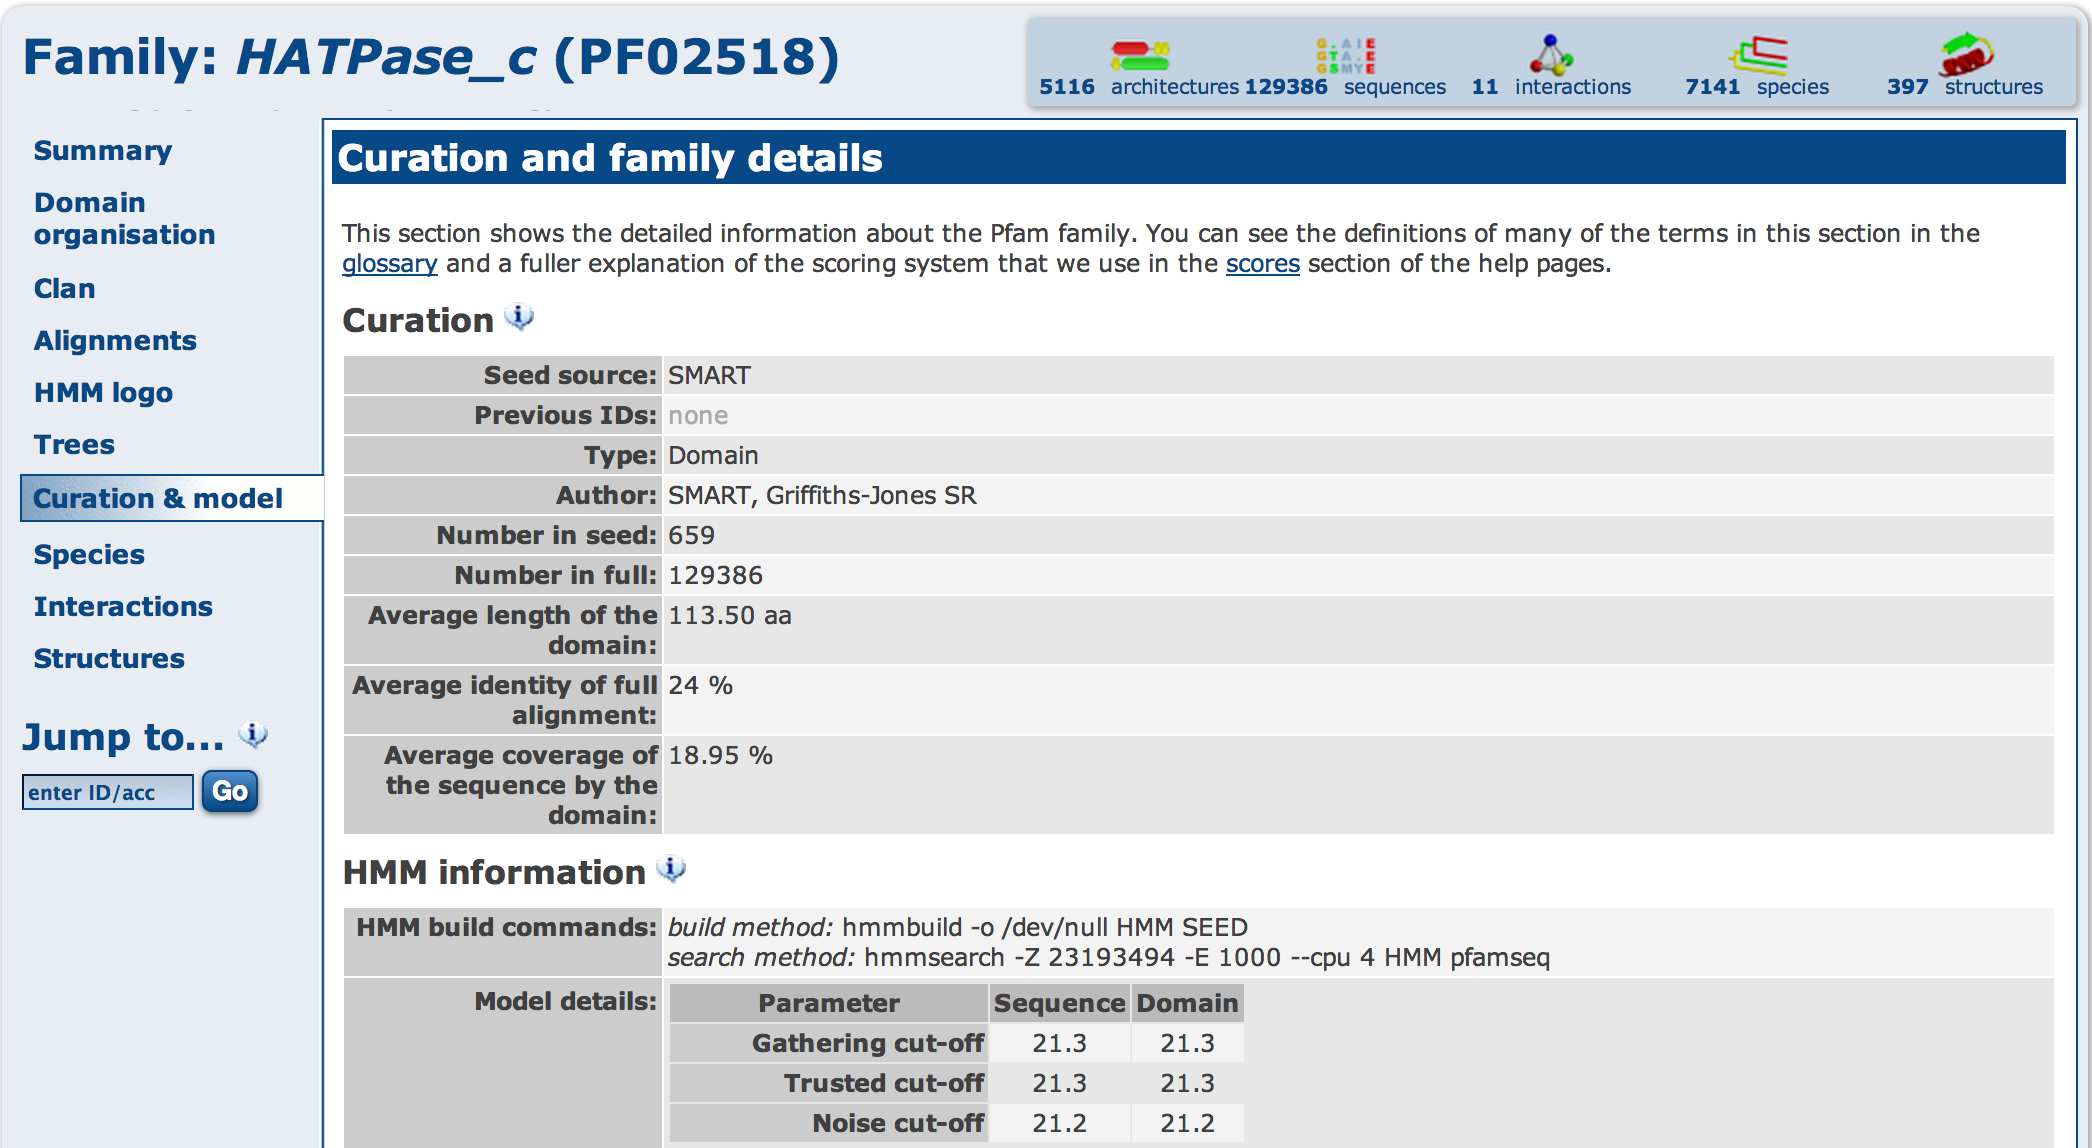
\includegraphics[width=0.8\textwidth]{images/pfam10} 
      \end{center}      
    \end{frame}

    \begin{frame}
      \frametitle{How PFam Works}   
      \begin{itemize}
        \item At the command-line, PFam works by running HMMer against published PFam databases
        \item Command-line use gives more control over HMMer settings, but less pretty output
        \item At the command-line, care must be taken over using GA, TC, NC cutoffs
      \end{itemize}
    \end{frame}

    % InterPro and RAST
    \subsection{InterPro and RAST}
    \begin{frame}
      \frametitle{InterPro}   
      \begin{itemize}
        \item Webserver for single sequences
        \item Local installations for whole-genome annotations
      \end{itemize}
      \begin{center}
        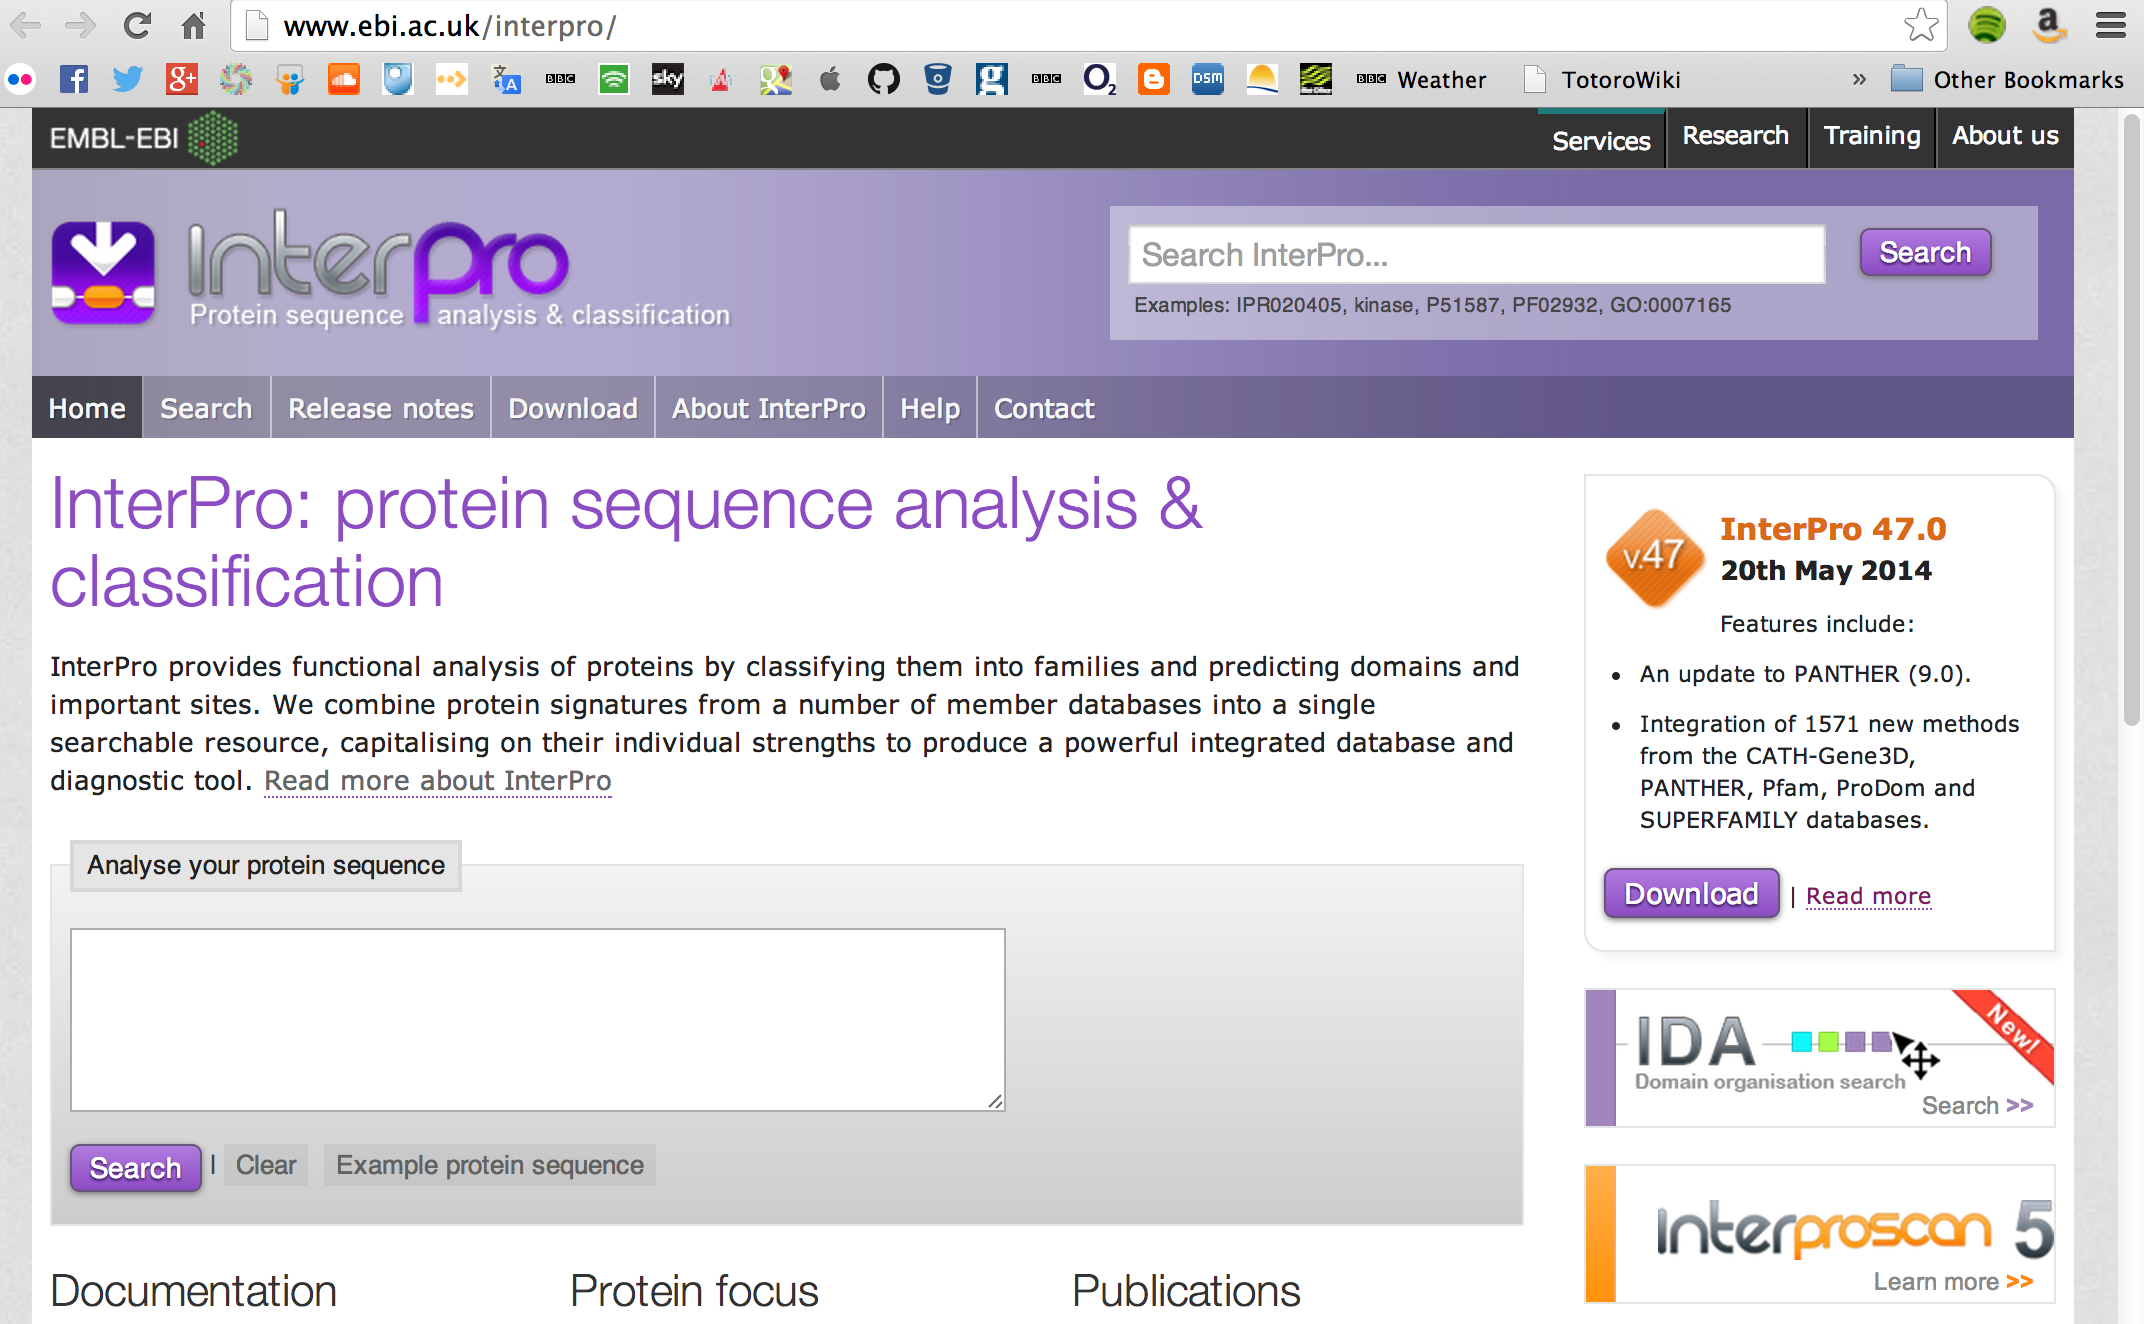
\includegraphics[width=0.8\textwidth]{images/interpro} 
      \end{center}        
    \end{frame}
    
    \begin{frame}
      \frametitle{How InterPro Works}   
      \begin{itemize}
        \item InterPro \url{http://www.ebi.ac.uk/interpro/} classifies proteins into families and predicts domains using a large number of tools, including:
        \begin{itemize}
          \item PFam, PROSITE, PRINTS, PANTHER, CATH
        \end{itemize}
        \item Predictive models of these databases are called `signatures'
      \end{itemize}
    \end{frame}

    \begin{frame}
      \frametitle{RAST}   
      \begin{itemize}
        \item Webserver for prokaryotic whole-genome annotation
        \item RAST calls genes as well as annotates them, but will accept your gene calls
      \end{itemize}
      \begin{center}
        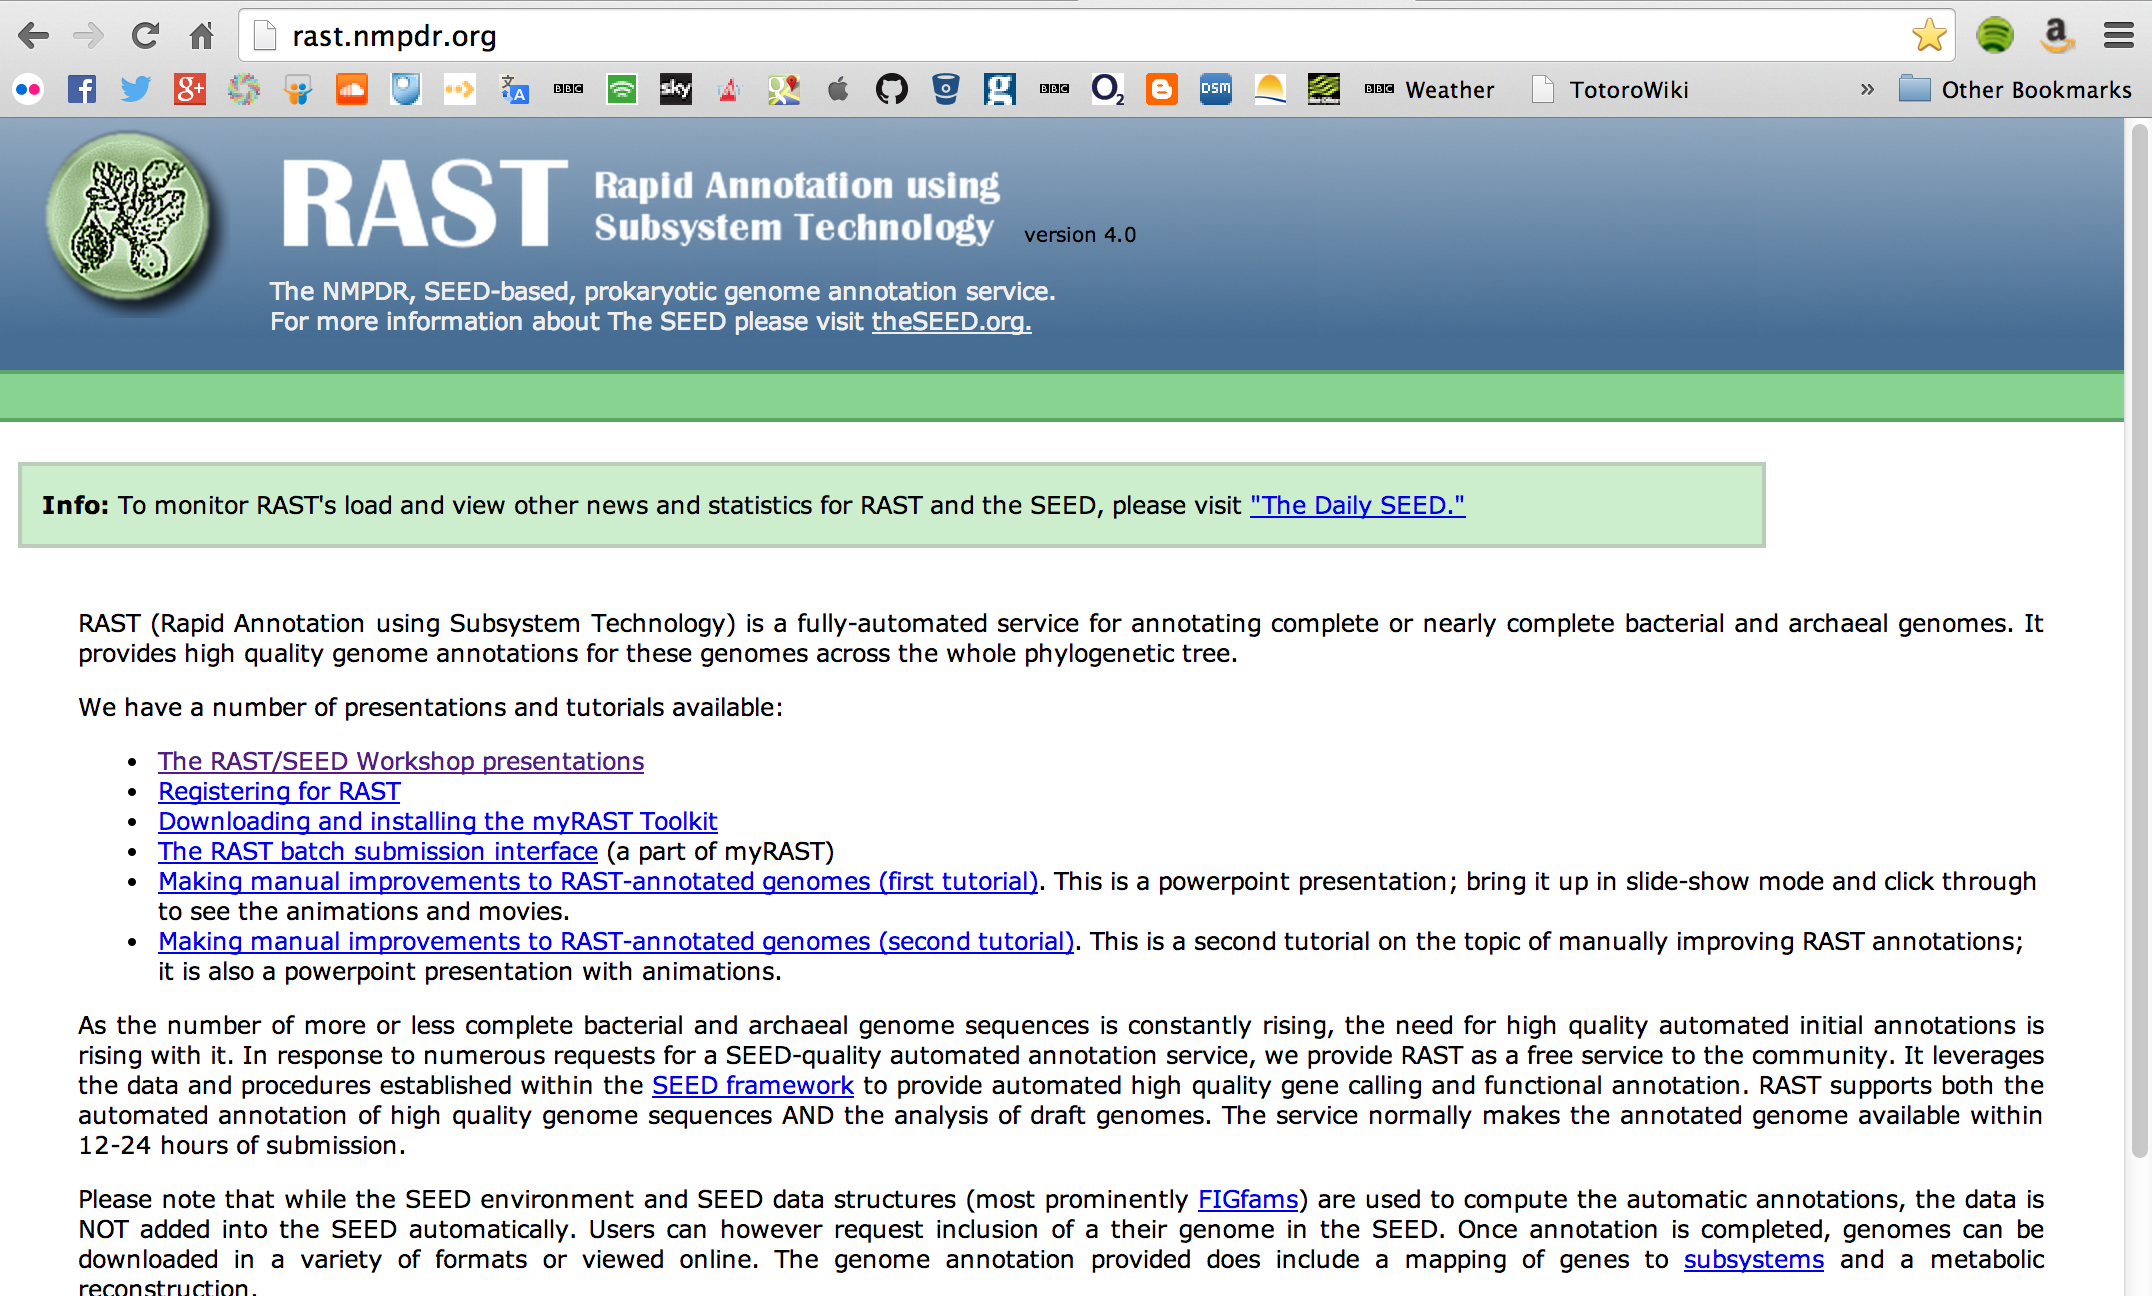
\includegraphics[width=0.8\textwidth]{images/rast} 
      \end{center}        
    \end{frame}

    \begin{frame}
      \frametitle{How RAST Works}   
      \begin{itemize} 
        \item Functional annotation is based on two SEED databases
        \begin{itemize}
          \item [A-SEED] Annotator SEED - representative high-quality
          \item [P-SEED] PATRIC-SEED - all prokaryotic genomes
        \end{itemize}
        \item SEEDs divided into FIGFams: families that are believed to implement the same function (isofunctional homologs)
        \item $k$-mer profile signatures are used to assign query sequences to FIGFams
      \end{itemize}
    \end{frame}

    \begin{frame}
      \frametitle{Your InterPro and RAST annotation data}
      We've already prepared these files for you:
      \begin{itemize}
        \item InterPro raw output: \texttt{chr*\_iprscan.raw}
        \item RAST output: \texttt{chr*\_RAST.gff}
      \end{itemize}
    \end{frame}

% [fragile] frames must end with \end{frame} directly following a newline, or they break!
  \begin{frame}[fragile]
    \frametitle{Visualisation of InterPro/RAST data in Artemis}
    InterPro raw output is not in a standard format
\begin{lstlisting}[language=bash]
$ head chrA_iprscan.raw 
chrA_04004	7A8F7B9C0479F48C	368	HMMPfam	PF06674	DUF1176	29	360	6.499999999999917E-49	T	23-Mar-2012	IPR009560	Protein of unknown function DUF1176	
chrA_04005	128211B8B939DE6B	365	HMMPfam	PF06674	DUF1176	32	358	1.2000000000000004E-61	T	23-Mar-2012	IPR009560	Protein of unknown function DUF1176	
chrA_04009	9E5C628D590CC7AE	1342	HMMPfam	PF04565	RNA_pol_Rpb2_3	513	582	1.4999999999999956E-29	T	23-Mar-2012	IPR007645	RNA polymerase Rpb2, domain 3	Molecular Function: DNA binding (GO:0003677), Molecular Function: DNA-directed RNA polymerase activity (GO:0003899), Biological Process: transcription, DNA-dependent (GO:0006351)
\end{lstlisting}
    Need to use \texttt{converter.pl} - skipping this for time
\end{frame}

% [fragile] frames must end with \end{frame} directly following a newline, or they break!
  \begin{frame}[fragile]
    \frametitle{Visualisation of InterPro/RAST data in Artemis}
    RAST will give us GFF, suitable for Artemis
\begin{lstlisting}[language=bash]
$ head chrA_RAST.gff
##gff-version 3
chrA	Prodigal_v2.00	CDS	3	1430	187.7	+	0	ID=chrA_00001;Alias=fig|556.22.peg.1;Name=Chromosomal replication initiator protein DnaA
chrA	Prodigal_v2.00	CDS	1435	2535	185.6	+	0	ID=chrA_00002;Alias=fig|556.22.peg.2;Name=DNA polymerase III beta subunit (EC 2.7.7.7);Ontology_term=KEGG_ENZYME:2.7.7.7
chrA	Prodigal_v2.00	CDS	2676	3761	146.2	+	0	ID=chrA_00003;Alias=fig|556.22.peg.3;Name=DNA recombination and repair protein RecF
\end{lstlisting}
\end{frame}

    \begin{frame}
      \frametitle{RAST}   
      GFF can be imported in the usual way
      \begin{center}
        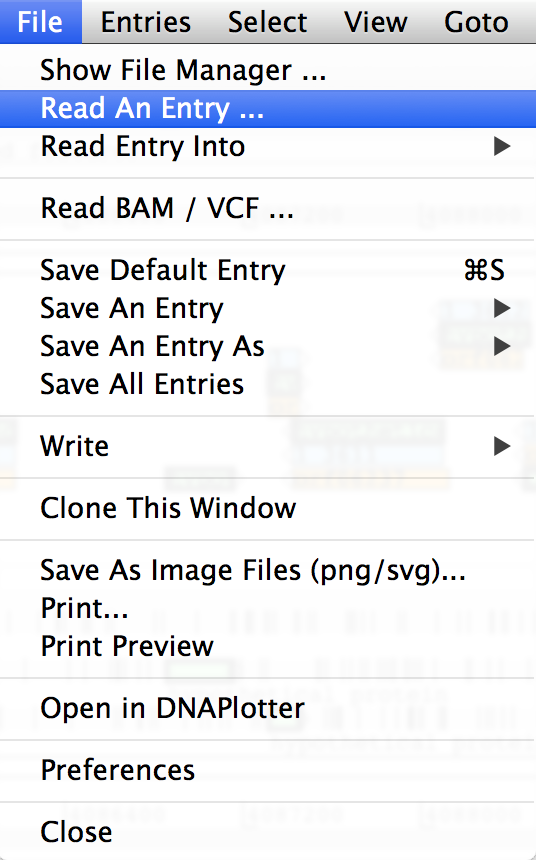
\includegraphics[width=0.3\textwidth]{images/rast0} 
      \end{center}        
    \end{frame}

    \begin{frame}
      \frametitle{RAST}   
      CDS predictions can be stacked
      \begin{center}
        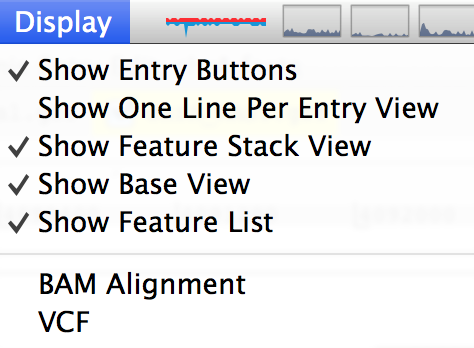
\includegraphics[width=0.4\textwidth]{images/rast1} 
      \end{center}        
    \end{frame}

    \begin{frame}
      \frametitle{RAST}   
      Predictions are in good agreement, and annotation visible
      \begin{center}
        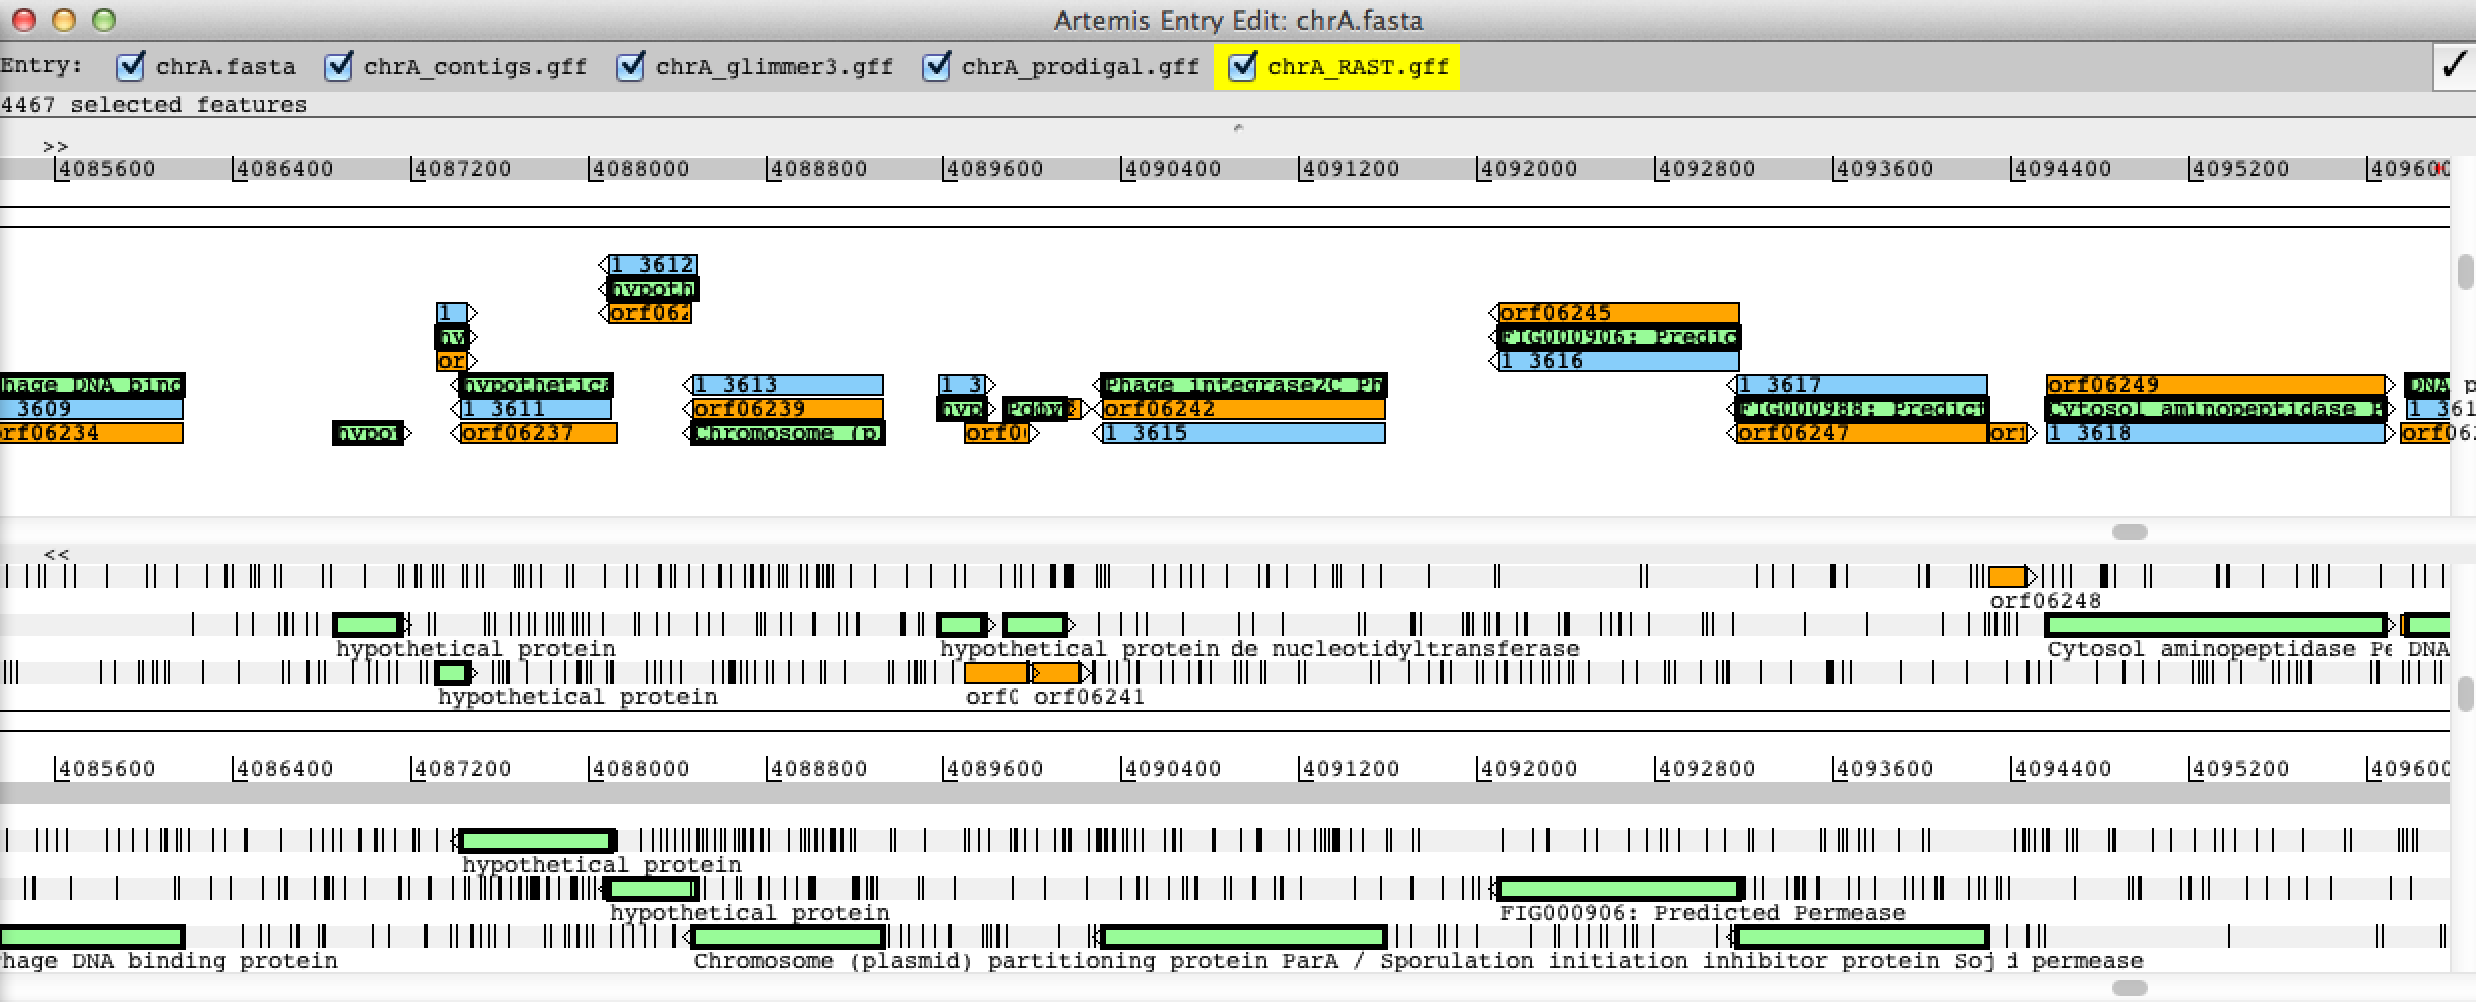
\includegraphics[width=0.9\textwidth]{images/rast2} 
      \end{center}        
    \end{frame}

    \begin{frame}
      \frametitle{Automated Functional Prediction}   
      \framesubtitle{Lessons learned}   
      \begin{itemize}
        \item Many alternative algorithms and databases are available 
        \item Integrated solutions (e.g. InterPro) are available
        \item Faster and larger-scale options tend to be more approximate
        \item How good is the agreement between alternatives?
        \item Automated annotations are a starting point, not a destination
      \end{itemize}
    \end{frame}

  % Gene Comparisons
  \section{Gene Comparisons}
    \begin{frame}
      \frametitle{Methods}   
      Most involve annotation transfer by sequence homology. \\
      Much is dependent on the quality of the alignment, and training set annotation.
      \begin{itemize}
        \item (Blast2GO \url{http://www.blast2go.com/b2ghome})
        \item (KEGG Automatic Annotation Server \url{http://www.genome.jp/kegg/kaas/})
        \item PFam \url{http://www.sanger.ac.uk/resources/databases/pfam.html}
        \item InterProScan \url{http://www.ebi.ac.uk/interpro/interproscan.html}
        \item RAST \url{http://rast.nmpdr.org/}
      \end{itemize}
    \end{frame}

    % BLAST/RBBH against known sequences to transfer function
    \subsection{BLAST}
% [fragile] frames must end with \end{frame} directly following a newline, or they break!
  \begin{frame}[fragile]
    \frametitle{Download Reference Sequences}
    Change directory to \texttt{chromosomes}, download reference protein data, and return to workspace
\begin{lstlisting}[language=bash]
$ wget ftp://ftp.ncbi.nih.gov/genomes/Bacteria/Pectobacterium_atrosepticum_SCRI1043_uid57957/NC_004547.faa
\end{lstlisting}
\end{frame}

    \begin{frame}
      \frametitle{Save CDS Annotation from Artemis}   
      Select all \texttt{prodigal} predicted CDS
      \begin{center}
        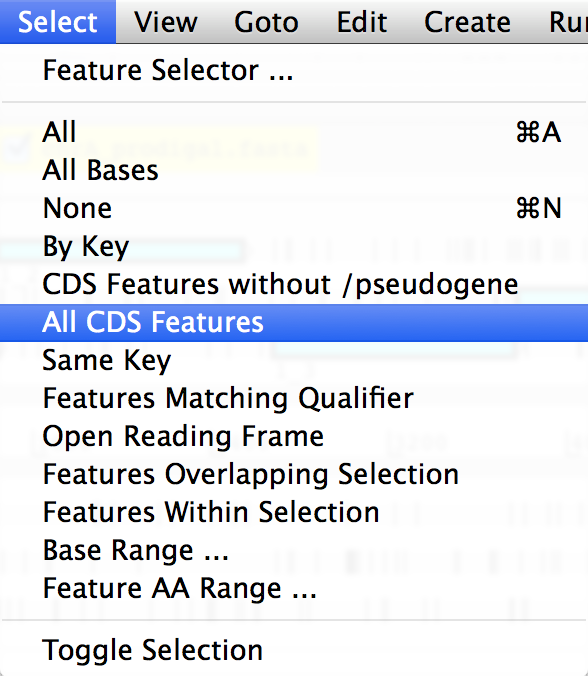
\includegraphics[width=0.6\textwidth]{images/export1}     
      \end{center}        
    \end{frame}

    \begin{frame}
      \frametitle{Save CDS Annotation from Artemis}   
      Choose to write protein sequences
      \begin{center}
        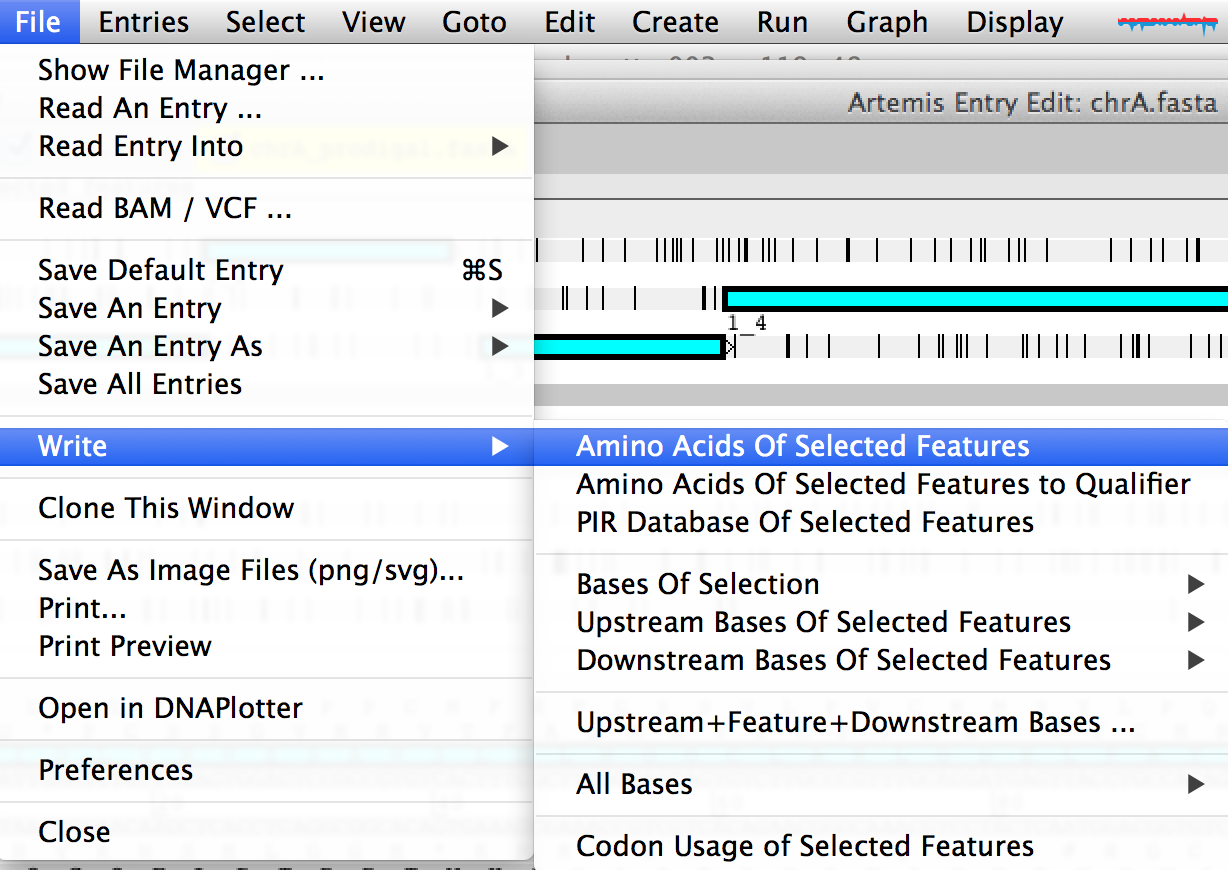
\includegraphics[width=0.6\textwidth]{images/export2}     
      \end{center}        
    \end{frame}

    \begin{frame}
      \frametitle{Save CDS Annotation from Artemis}   
      Select an output filename, e.g. \texttt{chrA\_prodigal.fasta}
      \begin{center}
        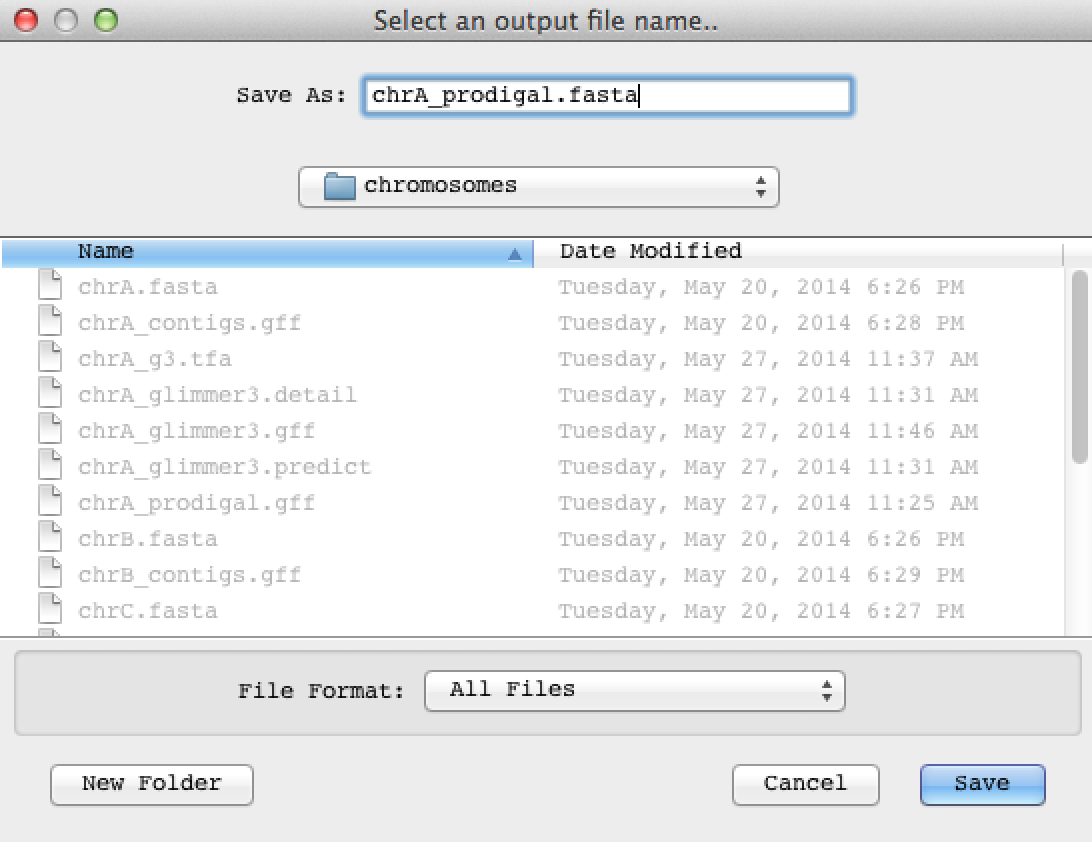
\includegraphics[width=0.6\textwidth]{images/export3}     
      \end{center}        
    \end{frame}


